Now that we've defined a selection of random processes, we can start discussing what might be appropriate to fit to our data. We'll define a particular emission model, simulate it, and then see what we can recover from it.

\section{Fitting a Non-Homogeneous Poisson Process}

The simplest place to start would be a homogeneous Poisson process, though a cursory glance at our data suggests that this would not be appropriate - the user is clearly tweeting at different rates at different times of day, and is not homogeneous. Let's try a non-homogeneous poisson process. We assume that the tweeter emits tweets according to an inhomogeneous poisson process, and attempt to find its rate function. For convenience, we'll describe our time in hours, though naturally the units could be arbitrary. We start by simulating a poisson process of known rate function, and seeing how well we can recover it. We start with a simple step function,

$$
\lambda(t) = 
\begin{cases}
5  & \mbox{for} \quad 0  \leqslant t < 30\\
10 & \mbox{for} \quad 30 \leqslant t < 50\\
5  & \mbox{for} \quad 50 \leqslant t < 100
\end{cases}
$$

And we simulate the process for 100 hours, producing a trace such as the one displayed in Figure \ref{trace_nonhom1}.

\begin{figure}[h]
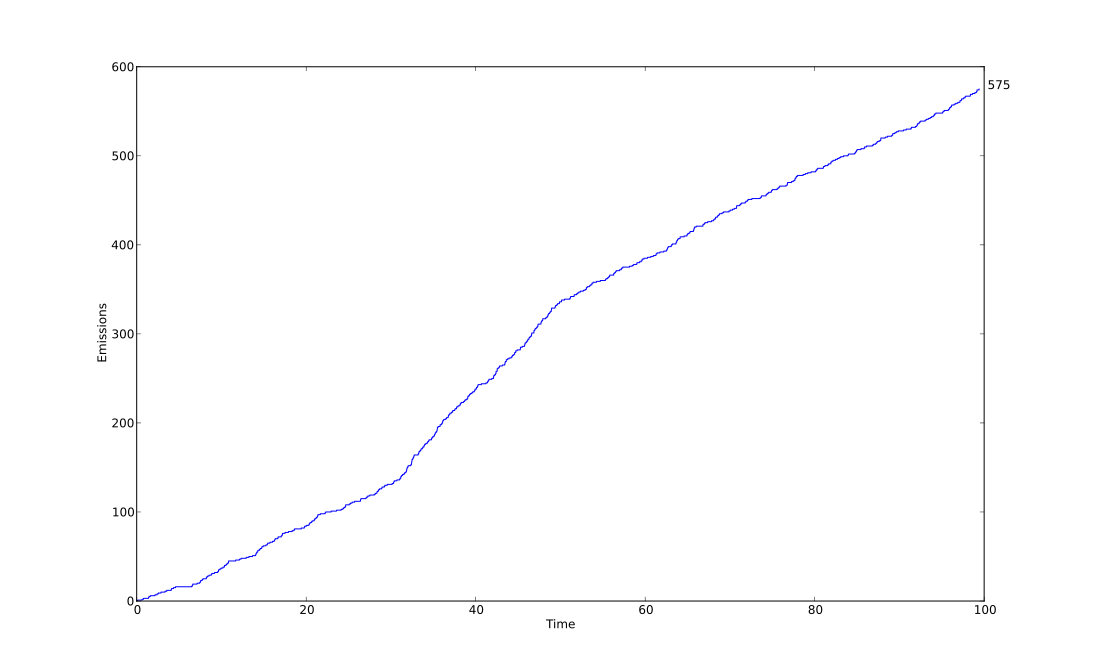
\includegraphics[width = \textwidth]{./images/trace_nonhom1.png}
\caption{A trace of an inhomogeneous Poisson process. Time flows along the x-axis, and the value on the y-axis shows the number of emissions seen thus far. A total of 575 emissions were observed.}
\label{trace_nonhom1}
\end{figure}

We can fit a step function by observing multiple traces of these poisson processes, taking the differences in emission times, then attempting to cluster them with the k-means algorithm%cite
. The average number of emissions per trace is the integral of the rate wrt time over the time interval for which we observe, ie if $N$ is the number of observed emissions in a single trace,

$$
\mathbb{E}(N) = \int^{100}_0 \lambda(t) \; dt = 600
$$

So if we run out 6 traces we'll observe roughly $3,600$ emissions, a little more than our real data set. Fitting a function to these gives us the results from Figure \ref{fit_nonhom1}

\begin{figure}[h]
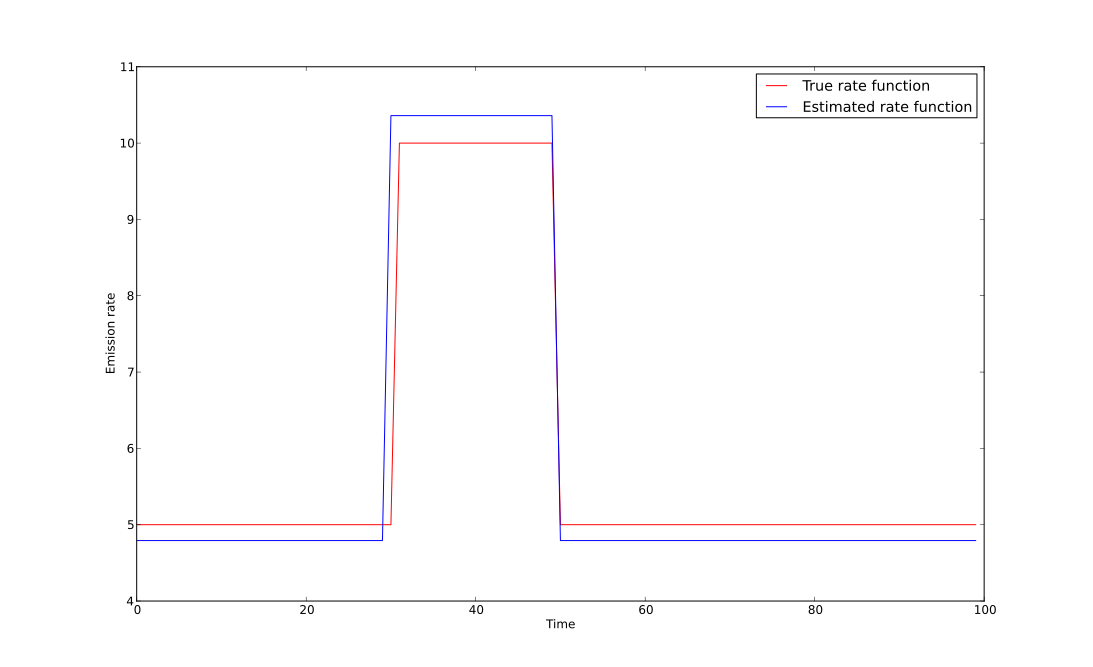
\includegraphics[width = \textwidth]{./images/fit_nonhom1.png}
\caption{An attempt to recover the rate function used to generate Figure \ref{fit_nonhom1}}
\label{fit_nonhom1}
\end{figure}

Eyeballing this, we see that it's not a terrible fit in this first attempt, but if we try a more complex rate function, %diagram
happens

%Lots of steps in a step function

We could instead attempt to fit a polynomial function but this requires more parameters, and ignores a somewhat worse problem, visible in %figure

% Trace of one day, showing bursts

We can see an important feature between 
%time1
and
%time2
. We'll call this a ``burst". The user is tweeting very rapidly for a short period of time. These bursts occur at random times throughout the day, and last for random lengths of time, but they all take on the same form. This heavily restricts our function. We can't simply say that at some particular time there is always a burst, but we also cannot deny their existence by smoothing them out since these bursts, by their very nature, will account for the majority of the observed tweets.

Clearly, a different approach is needed.

\section{Fitting a Markov-Modulated Poisson Process}

An MMPP seems ideal then, capturing the simplicity of a step function, and letting us model the idea of randomly distributed bursts throughout a day. Indeed, several authors have postulated that such a model would be ideal for simulating human behavior %lots of citations go here
but there have so far been no actual quantifiable studies of its relevance. Part of the reason for this is likely the lack of algorithms.

Fitting a Hiddin Markov Model of any kind relies on two main algorithms, Baum-Welch %cite
and Viterbi
%cite
. The Baum-Welch Algorithm is an expectation-maximisation algorithm for finding the transition probabilities/rates and the emission probabilities, given a set of possible emissions, a number of states to fit and an observed sequence of emissions. Viterbi will take an observed sequence of emissions and the parameters of an HMM, and produce the most likely state in which each of these emissions happened. The HiddenMarkov package hosted on CRAN \cite{hiddenmarkov}
is the only easily-accessible Hidden Markov Model package which supports the Markov Modulated Poisson Process, but does not contain any implementation of the Viterbi algorithm. We have two ways of working around this, either write our own or discretise the process.

Since the times between emissions in an MMPP are usually exponentially distributed, we could work in discrete time by letting $y_t$ be the time between the $t^{th}$ and $(t+1)^{th}$ emissions, though this sacrifices some information. We no longer consider the possibility of making multiple transitions between emissions, and ignore the intrinsic link between the times between emissions and the times between state transitions, but this model may also yield some useful results. We'll be trying out both of them.

\subsection{A derivation of the classical Viterbi algorithm}

The Viterbi algorithm for a standard Discrete Time Hidden Markov Model relies on a known, finite observation space $O$, a known distribution on $O$ for each state $s$, $p_s$, and known transition probabilities $\pi_i,j$, with known initial probabilities for each state $s$, $\delta_s$. We let $[k] = \{1,2,...,k\}$. The goal is, given a sequence of $T$ observations $(y_n)_{n \in [T]}$, $y_i \in Y$, to find the sequence of states $(x_n)_{n \in [T]}$ satisfying

$$
\mathbf{x} = \argmax_{\widehat{\mathbf{x}} \in S^T} \pr(\mathbf{\widehat{x}} | \mathbf{y})
$$

We call $\mathbf{x}$ the Viterbi Path.

We let $V_{t,s}$ be the probability of the most probable state sequence responsible for the first $t$ observations which ends in state $s$ %cite http://www.cs.cmu.edu/~epxing/Class/10701/Lecture/lecture12-HMM.pdf
. We have that $V_{1,s}$ is the probability of both being in state $s$ at time 1 and seeing observation $y_1$ from state $s$. A simple application of Bayes' Rule gives us that

$$
V_{1,s} = \pr (y_1|s)\pr(x_1=s)
$$

Recall that $\delta_s$ is the probability of being in state $s$ at time 1, ie $\pr(x_1=s)$, and that $p_s(y_1)$ is the probability of observing $y_1$ from state $s$, ie $\pr (y_1|s)$. In practice, these won't be known, but estimates of them will be given by the Baum-Welch algorithm, so we will use their maximum-likelihood estimates to give us,

$$
V_{1,s} = p_s(y_1)\delta_s
$$

Given $V_{\tau,s}$ for $\tau < t$, we can find $V_{t,s}$ by noting that the Markov Property implies a form of memorylessness. Given the present, the future is conditionally independent of the past. As such, we need only consider $V_{t-1,s}$ for each $s$, as well as our known parameters. 

The probability of the most likely path that leads us to state $s$ at time $t$ is given by the probability of the most likely path that led us to $s'$ at time $t-1$, and then jumped to $s$ at time $t$, and then emitted $y_t$ from state $s$. The probability of jumping from $s'$ to $s$ is $\pi_{s',s}$. The probability of emitting $y_t$ from state $s$ is $p_s(y_t)$. The probability of the most likely path that leads us to $s'$ at time $t-1$ is $V_{t-1,s'}$. Hence,

$$
V_{t,s} = p_s(y_t) \max_{s'\in S} (\pi_{s',s}V_{t-1,s'})
$$

Using this recurrence, we can find $V_{t,s} \forall t \in [T]$ by a standard dynamic programming algorithm.

From here, we can then work backwards to find the Viterbi path. $x_T = \argmax_{s \in S} V_{t,s}$ - the most likely final state is the state in which the path of maximum probability ends.

Let
 
$$
T_{t,s} = \argmax_{s'\in S}(\pi_{s',s}V_{t-1,s'})
$$

Ie, $T_{t,s}$ is the state from which we are most likely to have come at time $t-1$ given that we are in state $s$ at time $t$, we can then see that $x_{t-1} = T{x_t,t}$. Note the similarities in the definitions of $V$ and $T$ - both can be calculated simultaneously - $V$ is the maximum, $T$ is the argument that maximises. $T_{1,s}$ is never used, so need never be defined. 

Since we have an expression for $x_{t-1}$ in terms of $x_t$, and for $x_T$, we can then recover $\mathbf{x}$, the Viterbi Path. \ref{algvitdthmm} defines this algorithm.

\begin{algorithm}
\SetAlgoLined
\SetKwInOut{Input}{input}
\SetKwInOut{Output}{output}

\caption{The Viterbi Algorithm for DTHMMs}\label{algvitdthmm}
\KwData{$(S,\delta,\Pi,O,p)$, a DTHMM}
\Input{$\mathbf{y}$, an observed sequence of $T$ emissions, indexed from $1$ to $T$}
\Output{$\mathbf{x}$, the most likely sequence of states generating these emissions}

\Begin{
	\For{$s \in S$}{
		$V_{1,s} <- p_s(y_1)\delta_s$
	}
	\For{$t \leftarrow 2$ \KwTo $T$}{
		\For{$s \in S$}{
			$V_{t,s} <- p_s(y_t) \max_{s' \in S}(\pi_{s',s}V_{t-1,s'})$ \\
			$T_{t,s} <- \argmax_{s' \in S}(\pi_{s',s}V_{t-1,s'})$
		}
	}
	$x_T <- \argmax_{s' \in S}(V_{s',T})$\\
	\For{$t \leftarrow T$ \KwTo $2$}{
		$x_{t-1} <- T_{x_t,t}$
	}
	\KwRet{$\mathbf{x}$}
}
\end{algorithm}

\subsection{A First Approximation of the Viterbi Algorithm for the Markov-Modulated Poisson Process}

Recall the dependencies for the DTHMM Viterbi Algorithm. We require knowledge of a finite $O$, $p_s$ for each $s$, and $\pi_{ij}$ for each pair of states $i,j$.

In an MMPP, we observe a Poisson Process of rate randomly varying between various known rates - the rates being our states. Let $S = \{\lambda_1,...,\lambda_m\}$. Our observations can be interpreted as exponential random variables of these rates. Let $\tau_0 = 0$, and $\tau_i$ be the time of the $i^{th}$ poisson emission for $i \in [n]$. Let $y_i = \tau_i-\tau_{i-1}$ for $i \in [n]$. Given that the underlying CTMP was in state $\lambda_s$ at time $\tau_i$, we have that $y_i \sim Exp (\lambda_s)$. From the properties of the generic CTMP, the probability that the process is in state $j$ at time $\tau_i$ given that it was in state $i$ at time $\tau_{i-1}$ is given by $(e^{Qy_i})_{\lambda_{i},\lambda_{j}}$. To ease notation, we'll write this as $(e^{Qy_i})_{i,j}$, omitting the $\lambda$s.

The state space $S$ and transition rates $Q$ are estimated by the Baum Welch algorithm as before, so after running Baum Welch over an observed trace, we can start to find the most likey state at each emission. Note that this ``Viterbi Path" is not the most likely sequence of state transitions, it is instead the most likely state in which the underlying CTMP resides at the time of each emission. This quirk is discussed in %APPENDIX REF

Since our emissions are continuous, we don't have any notion of ``most probable" - if we model height continuously, the probability that I meet someone exactly 1.8m tall is the same as the probability that I meet someone exactly 18m tall, they're both 0 - so instead we'll base our likelihood calculations off probability density - capturing the idea that, even though I don't know for certain that I'll meet one of the two, it's more likely for me to meet the 1.8m tall person.

We let $p_s(t)= \lambda_s e^{-t\lambda_s}$, the probability density of an exponential random varaible of rate $\lambda_s$ evaluated at $t$. Let $V_{t,s}$ be the probability density of the most likely path that leads us to emitting $y_t$ from state $s$. We have that

$$
V_{1,s} =  \delta_{s}p_s(y_1)
$$

The probability density of the most likely path that leads us to waiting for time $y_1$ before making an emission is given by the probability of starting in state $s$, multiplied by the probability density of waiting $y_1$ for an emission from state $s$. The memorylessness property of a CTMP allows us to only consider $V_{t-1,s}$ when calculating $V_{t,s}$. We have that

$$
V_{t,s} = p_s(y_t) \max_{s'\in S} (V_{t-1,s'}(e^{Qy_t})_{s',s})
$$

The probability density of the most likely path that leads us to waiting for time $y_t$ between the $(t-1)^{th}$ and $t^{th}$ emissions in state $s$ is given by the probability density of the most likely path that takes us to state $s'$ for the $(t-1)^{th}$ emission, followed by jumping (along any arbitrary path) into state $s$ for emission $t$, multiplied by the probability density of emitting $y_t$ in state $s$.

From here, we can proceed as normal. We define $T$ as before to record our most likely states at each transition, and work backwards to find $\mathbf{x}$, producing the following algorithm

\begin{algorithm}
\SetAlgoLined
\SetKwInOut{Input}{input}
\SetKwInOut{Output}{output}

\caption{An Approximate Viterbi Algorithm for MMPPs}
\KwData{$(S,\delta,Q,p)$, an MMPP}
\Input{$\mathbf{y}$, the absolute times of an observed sequence of $T$ emissions, indexed from $1$ to $T$}
\Output{$\mathbf{x}$, the most likely sequence states in which the underlying CTMP resides for each emission in $\mathbf{y}$}

\Begin{
	\For{$t <- 2$ \KwTo $T$}{
		$\tau_{t-1} <- y_t-y_{t-1}$
	}
	$T <- T-1$
	\For{$s \in S$}{
		$V_{1,s} <- p_s(t_1)\delta_s$
	}
	\For{$t \leftarrow 2$ \KwTo $T$}{
		$A <- e^{Q\tau_t}$
		\For{$s \in S$}{
			$V_{t,s} <- p_s(\tau_t) \max_{s' \in S}(A_{s',s}V_{t-1,s'})$ \\
			$T_{t,s} <- \argmax_{s' \in S}(A_{s',s}V_{t-1,s'})$
		}
	}
	$x_T <- \argmax_{s' \in S}(V_{s',T})$\\
	\For{$t \leftarrow T$ \KwTo $2$}{
		$x_{t-1} <- T_{x_t,t}$
	}
	\KwRet{$\mathbf{x}$}
}
\end{algorithm}

The reason that this is an approximation is the fact that the algorithm assumes that either a jump happens instantaneously, or not at all - we always evaluate $p_s(y_t)$, rather than $p_s(y_t-\tengt)$\footnote{\tengt - tinco - represents the voiceless alveolar stop in the Tengwar alphabet, as devised by JRR Tolkein. When dealing with time so frequently, we eventually run out of ways to write the letter t}, where $\tengt$ represents the time we wait for all the relevant transitions to occur. The times between state transitions are exponentially distributed, and we are dealing with the most likely outcomes. The most likely outcome of any exponential distribution is $0$ so, if the underlying CTMP jumps from one state to another, the most likely time for that jump to happen is immediately, so $\tengt = 0$. If multiple jumps happen, their individual times are exponentially distributed, but their sum does not have a mode of 0.

This first approximation is in fact very powerful. Approximating in this way assumes that multiple transitions between emissions are rare, alternatively  that emissions within each state are more frequent than transitions out of that state. If the converse is true - transitions out of the state are more frequent than emissions within the state - then we have an odd situation whereby some state is frequently entered and then left again with no emissions happening. Whilst such states are perfectly valid and can indeed exist in a theoretical MMPP, detecting one in reality with no prior knowledge is very difficult.

As a final note, we can further refine the fitted model based on the results of the Viterbi algorithm by changing the estimated rate of each state to the observed rate of the emissions estimated to occur in that state. By the nature of these estimation algorithms, these results are likely to differ, and with a large sample size what we observe is usually closer to the truth than what we assert.

\subsection{Applying the Algorithm}

%Put python stuff somewhere else

The algorithm was written in R and added to the pre-existing HiddenMarkov \cite{hiddenmarkov}
package, which was then recompiled to be loaded into an R environment. A Python script was written to call into this library from a more conveneint language using RPy2 %cite
, with mathematical, statistical and visualisation functions loaded from matplotlib\cite{matplotlib}, NumPy and SciPy.

As before, we first simulate a model, then see if we can recover it. The simulated model had the following parameters;

\begin{align*}
(\lambda_1,\lambda_2,\lambda_3) &= (0.01,0.5,2)\\
S &= \{\lambda_1,\lambda_2,\lambda_3\}\\
Q &= \bordermatrix{      & \lambda_1 & \lambda_2 & \lambda_3\cr
                \lambda_1 & \frac{-1}{20} & \frac{1}{60}  & \frac{1}{30} \cr
                \lambda_2 & \frac{1}{10}  & \frac{-2}{15} & \frac{1}{30} \cr
                \lambda_3 & \frac{1}{10}  & \frac{1}{60}  & \frac{-7}{60}\cr
			}\\
\delta &= \left(\frac{1}{3},\frac{1}{3},\frac{1}{3}\right)
\end{align*}

The expected course of an MMPP is somewhat harder to calculate, but 6,000 hours gave a similar number of emissions to the number of emissions in our data. The resulting trace can be seen in Figure \ref{trace_mmpp1}.

\begin{figure}[h!]
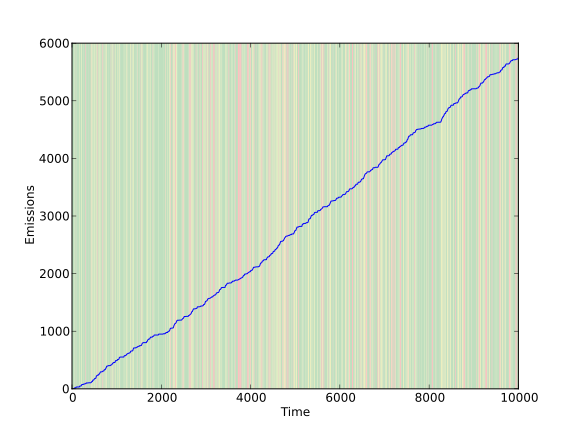
\includegraphics[width = \textwidth]{./images/trace_mmpp1.png}
\caption{A trace of an MMPP with the states shaded in colour}
\label{trace_mmpp1}
\end{figure}

Running the Baum-Welch algorithm over the trace with a known state size of 3 for 208 iterations, at which the model converged sufficiently, gives us the following predictions, rounded to 2 significant figures;

\begin{align*}
(\lambda_1,\lambda_2,\lambda_3) &= (0.0066,0.53,2.00)\\
S &= \{\lambda_1,\lambda_2,\lambda_3\}\\
Q &= \bordermatrix{      & \lambda_1 & \lambda_2 & \lambda_3\cr
                \lambda_1 & -0.061 & 0.022 & 0.039 \cr
                \lambda_2 & 0.10 & -0.14 & 0.053 \cr
                \lambda_3 & 0.094 & 0.020 & -0.11 \cr
			}\\
\delta &= (1.00,0.00,0.00)
\end{align*}

On inspection, most these parameters give a reasonable approximation of the originals, but $\delta$ seems to be well off the mark. The reason for this is fairly simple - the simulated trace had to start somewhere, and in this case it started in state 1. The algorithm was only given one trace, so to minimise the probability of error, it estimated that the underlying CTMP always starts in the state in which it was estimated to start. The initial distribution of the underlying CTMP isn't hugely relevant, however. We're interested in how the user tweets in the long term, and regardless of initial distribution this markov chain will reach an invariant distribution.

Running the modified viterbi algorithm over the process gives the estimate in Figure \ref{fit_mmpp1}

\begin{figure}[h!]
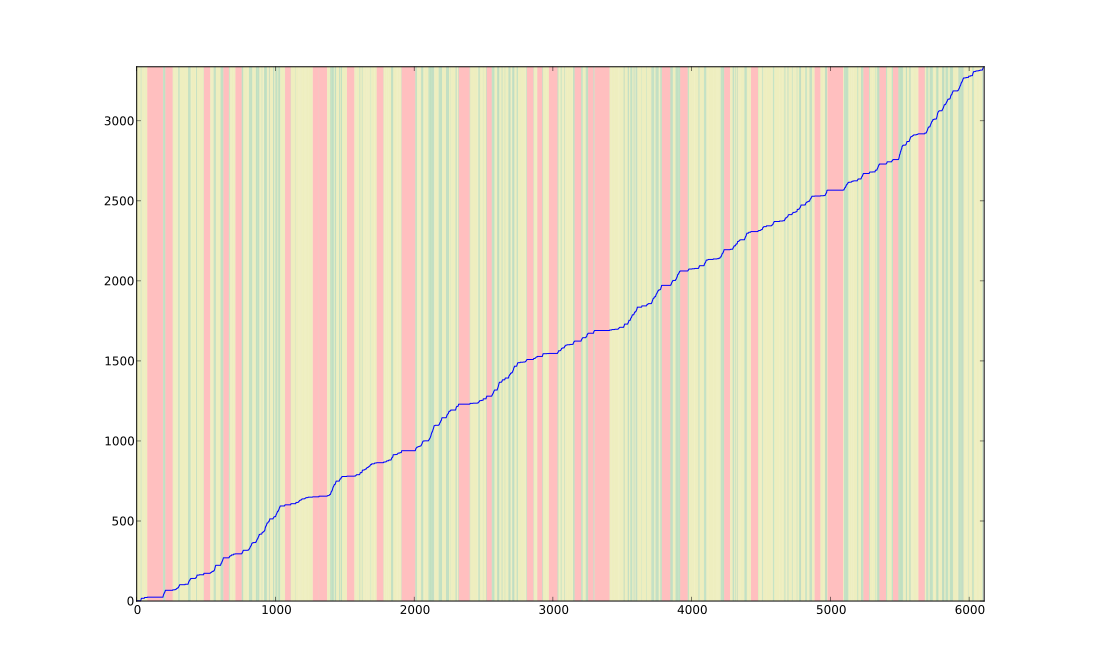
\includegraphics[width = \textwidth]{./images/fit_mmpp1.png}
\caption{The same trace as Figure \ref{trace_mmpp1}, but with the shading to match estimated states, rather than actual states}
\label{fit_mmpp1}
\end{figure}

Comparing the estimated path to the original in a way that clearly displays the results seems daunting, but we can do this in what I find a fairly beautiful way by simply aligning the two traces along the same scale, rendering them as bitmaps, then taking the difference in the colours between the two images using GIMP
%gimp.org
%http://docs.gimp.org/en/gimp-concepts-layer-modes.html
. Any black pixels are locations where the original two images match perfectly, all others are mistakes. Stripping the top row of colours will show mistakes over time. %diagram goes somewhere near here
. Figure \ref{compare_mmpp1} is a black and white thresholded version of the above, where all colours appear as white lines. The image is 91.2\% black so my estimated model matches the simulation 91.2\% of the time.

\begin{figure}[h!]
\includegraphics[width = \textwidth]{./images/compare_mmpp1.png}
\caption{A comparison between the estimated state sequences of Figures \ref{trace_mmpp1} and \ref{fit_mmpp1}. Matching areas are back, differing areas are white, and the axis is in red for clarity.}
\label{compare_mmpp1}
\end{figure}

Now that we've verified that our algorithms are capable of recovering known MMPPs to a high degree of accuracy, it's time to pump our data into it.

The data was preprocessed such that rather than recording exact times and dates of tweets, it instead recorded time since the beginning of the observation in hours at which each tweet occured. This was then fed into a HiddenMarkov MMPP, over which BaumWelch and Viterbi were then run based on the assumption of 3 states. The resulting model was as follows:
\clearpage
\begin{align*}
(\lambda_1,\lambda_2,\lambda_3) &= (0.0289,1.28,15.5)\\
S &= \{\lambda_1,\lambda_2,\lambda_3\}\\
Q &= \bordermatrix{      & \lambda_1 & \lambda_2 & \lambda_3\cr
                \lambda_1 & -0.123 & 0.120 & 0.004 \cr
                \lambda_2 & 0.441 & -1.09 & 0.648 \cr
                \lambda_3 & 0.00 & 5.25 & -5.25 \cr
			}\\
\delta &= (1.00,0.00,0.00)
\end{align*}

And, with the states shaded in in the colours represented above, the transitions were as represented in Figure \ref{fit_mmpp2}

\begin{figure}[h!]
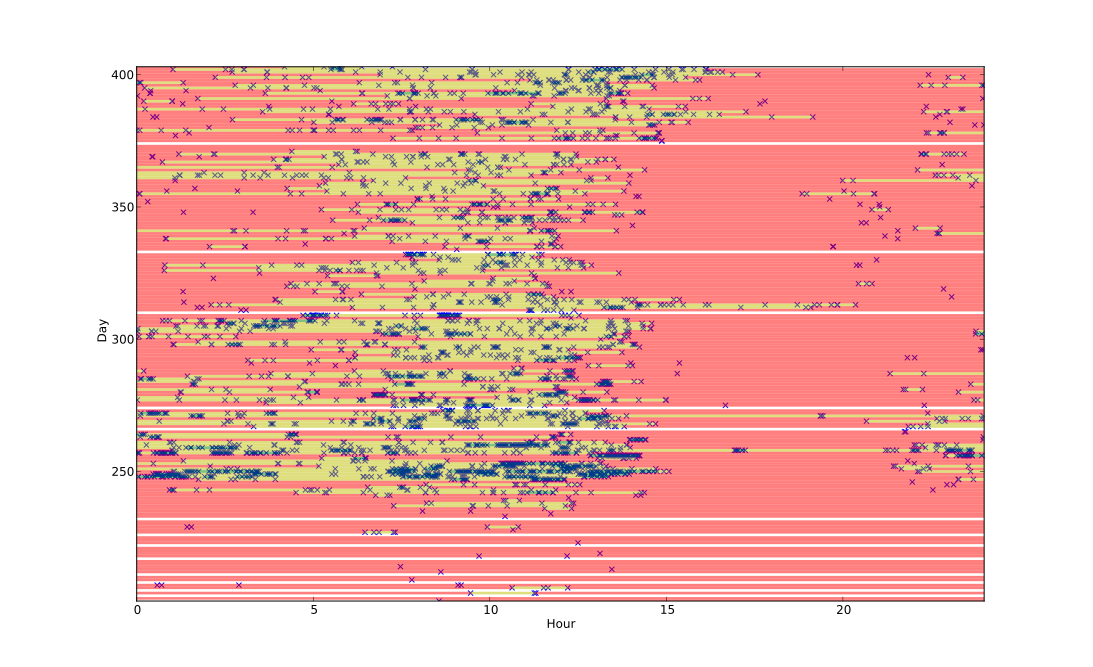
\includegraphics[width = \textwidth]{./images/fit_mmpp2.png}
\caption{The twitter data, with predicted states shaded - $\lambda_1$ in red, $\lambda_2$ in yellow, $\lambda_3$ in green. Since $\lambda_3$ is a burst state which only lasts for 12 minutes and contains several tweets, it can be difficult to see behind those tweets}
\label{fit_mmpp2}
\end{figure}

From this distance, we already see at least some kind of sensible behavior - the user seems to have regular sleeping patterns, tweeting during the day and not tweeting at night-time. Zooming in on a single day, we see some more sensible results - the burst mentioned before has been noticed and highlighted, and the normal day-to-day tweets all remain in the same state. The three states correspond to intuitive states for a human to occupy - in state $\lambda_1$ the user is asleep or otherwise away from the computer, tweeting roughly once every 50 hours, but only staying there for about 10 hours. In state $\lambda_2$, the user is awake, online, and going about his day as usual - as an active twitter user he tweets about 1.3 times per hour. Roughly every hour, the user will then either go to bed with probability ~$0.4$, or enter into a conversation with someone and produce a burst with probability ~$0.6$ - bursts are tweets produced at a rate of 15 per hour, or one every 4 minutes, and last around 12 minutes on average. This all seems fairly reasonable, though the probabilities of of the transitions out of the awake state seem

We can evaluate this model by performing a Kolmogorov-Smirnov test on the data for each state. It should follow an exponential distribution. Running this test, we find, however, that it very much does not - the p-values for each state were less than $2.2 \times 10^{16}$ - to say that this is low would be an understatement.

Whilst 3 states makes sense intuitively, there's no reason why this is definitely the case, so let's try different numbers of states. We can find the most optimal number based on the Bayesian Information Criterion %cite
Given an estimated model, we can define the Bayesian Information Criterion, $BIC$, as

$$
BIC = -2 \ln L + k \ln n
$$

Where $\ln L$ is the log-likelihood of the fitted model, ie the natural logarithm of the probability of observing the data given that the model is correct, $k$ is the number of parameters in the model, and $n$ is the number of data points used to fit the model.

An MMPP of $s$ states has $k=s^2+s-1$ free parameters - $Q$ contains $s^2$ elements, but each of the $s$ diagonal elements can be determined by the row on which it resides, we fit $s$ states, each of which is freely choosable, and $\delta$ has $s$ elements, one of which can be determined from the other $s-1$. The number of data points is the number of tweets we've observed, and the log likelihood is given by the Baun-Welch algorithm.

675 iterations of Baum-Welch were run over the data until a local optimum was reached. This optimum occured at 4 states with a BIC of 1470, described as follows:

\begin{align*}
(\lambda_1,\lambda_2,\lambda_3,\lambda_4) &= (0.0223,0.511,6.14,28.3)\\
S &= \{\lambda_1,\lambda_2,\lambda_3,\lambda_4\}\\
Q &= \bordermatrix{      & \lambda_1 & \lambda_2 & \lambda_3 & \lambda_4\cr
                \lambda_1 & -0.111 & 0.0950 & 0.0160 & 0.000 \cr
                \lambda_2 & 0.262  & -1.21  & 0.950  & 0.000 \cr
                \lambda_3 & 0.287  & 2.94   & -3.67  & 0.445 \cr
                \lambda_4 & 0.000  & 0.000  & 5.56   & -5.56 \cr
			}\\
\delta &= (1.00,0.00,0.00,0.00)
\end{align*}

Fitted by the same methods, we see the following results

\begin{figure}[h!]
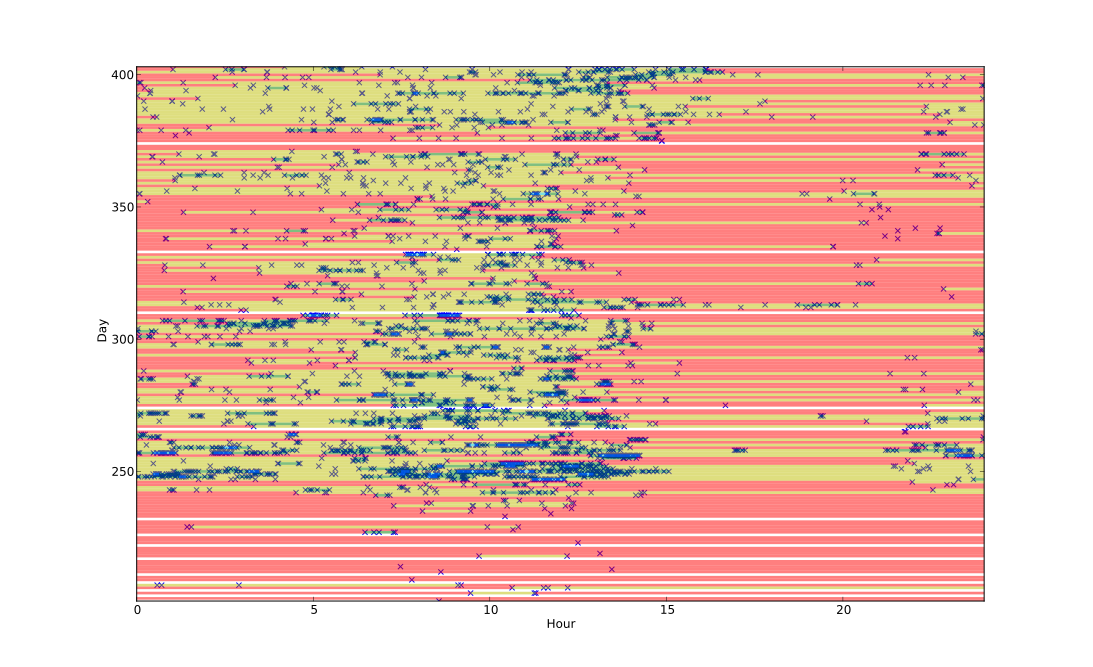
\includegraphics[width = \textwidth]{./images/fit_mmpp3.png}
\caption{The twitter data, with predicted states shaded - $\lambda_1$ in red, $\lambda_2$ in yellow, $\lambda_3$ in green and $\lambda_4$ in cyan. As with $\lambda_3$ in Figure \ref{fit_mmpp1}, $\lambda_4$'s emissions can be difficult to see.}
\label{fit_mmpp2}
\end{figure}

Unfortunately, the Kolmogorov-Smirnov tests still fail - the greatest p-value for any state was $3.85 \times 10^{-6}$. Fitting more states would probably give a better fit, but due to the quadratic scaling it would also start sending the number of parameters up to absurd levels - the Bayesian Information Criterion would not improve. This is the best MMPP we can fit, and it still isn't very good.

\subsection{An Alternative Approach}

From this point, it is starting to seem like the tweeter does not follow an MMPP, but there is one last thing we can attempt in this vein. A DTHMM can still have a continuous observation space and all the previous methods will work, just with probability density in place of probability. Rather than observing a series of times, we will instead observe a series of time differences, and look for any small number of states that lets us gather these differences into the same exponential distribution. The results from such a model will be similar, but lose some information about how long our tweeter actually spends in each state. The crucial difference between the two is that in an MMPP emissions and transitions take place along the same timeline - compare the Viterbi algorithms for both the MMPP and DTHMM, and note that the transition probabilities between a DTHMM's states do not depend on the observed emissions, whilst the transition probabilities in the MMPP version do.

So we go through the same procedure again - the intuitive 3 states didn't result in anything worthwhile, so we apply the old BIC test again to arrive at an optimum of 5 states and a BIC of 1446, resulting in a DTHMM with the following parameters;

\begin{align*}
S &= \{1,2,3,4,5\}\\
(\lambda_1,\lambda_2,\lambda_3,\lambda_4,\lambda_5) &= (0.108, 1.18, 4.27, 14.8, 32.4)\\
\delta &= (1,0,0,0,0)\\
\Pi &= 
\left(
    \begin{matrix}
    0.295 & 0.380 & 0.000 & 0.312 & 0.013 \\
    0.153 & 0.573 & 0.006 & 0.268 & 0.000 \\
    0.051 & 0.052 & 0.579 & 0.156 & 0.161 \\
    0.176 & 0.250 & 0.286 & 0.260 & 0.027 \\
    0.007 & 0.000 & 0.196 & 0.012 & 0.785
    \end{matrix}
\right)\\
Y &= \mathbb{R}^{+}\\
s \in S, y \in Y &=> p_s(y) = \lambda_s e^{-\lambda_sy}\\
\end{align*}

And finally perform some new KS tests to find one p-value of 0.03, and four others below $10^{-7}$.

From this, we can definitively conclude that the data cannot be well-clustered into a small number of exponentially distributed subsets. We can then conclude that these data do not follow any kind of simple poisson process, in spite of appearances.

\section{A Zoo of Problems}

Whilst this gives a fairly strong negative result that this tweeter is not a poisson process, it doesn't give any real explanation as to why. What went wrong? Inspecting the fitted models we see that the first few emissions don't quite fit in with the rest, but removing these anomalous results does little to the results of the Kolmogorov-Smirnov tests, they remain heavily negative in all cases.

Let's start looking at the emissions estimated to occur in each state. Since the DTHMM gave slightly better p-values, we'll use that as a jumping-off point.

% Density graphs here

And now we see an issue. The fits are close, but the heads of the distributions are light and their tails heavy. Indeed, on inspection, the observed emissions within each state seem closer to a low-variance lognormal distribution - if $X$ follows a lognormal distribution, then $\log(X)$ follows a normal distribution %cite mathworld
. Plotting a lognormal density curve alongside the observed curve, we see a somewhat closer fit, even though we attempted to fit these data to an exponential distribution. Let's try doing this properly.

Summing lognormal distributions into some stochastic process in the same way that we sum exponential distributions into a poisson process carries all manner of problems, however. The lognormal distribution is not memoryless, so the resulting processes within each state will be non-markovian, meaning that simple fitting algorithms like Baum-Welch and Viterbi require much more sophisticated modifications to work correctly.

We can, however, fit a discrete model to the data using a DTHMM with lognormal emissions, so let's do that. We take the natural logarithm of all the differences in emission times, fit multiple models and evaluate their BICs. Here, each state requires 2 parameters, a mean and a standard deviation, so the number of free parameters in an s-state model is now $s^2+2s-1$. We find that the optimal number of states is 3, and go ahead again with the KS tests, correcting the parameters for the estimated emissions within each state, resulting in p-values of 0.309, 0.174 and 0.413. At last, we have some statistically significant results, with the following parameters;

\begin{align*}
S &= \{1,2,3\}\\
(\mu_1, \mu_2, \mu_3) &= (-3.39, -1.43, 2.42)\\
(\sigma_1, \sigma_2, \sigma_3) &= (1.48, 1.79, 0.273)\\
\delta &= (0,1,0)\\
\Pi &= 
\left(
	\begin{matrix}
     0.924 & 0.070 & 0.006 \\
     0.005 & 0.903 & 0.049 \\
     0.000 & 0.865 & 0.135
	\end{matrix}
\right)\\
Y &= \mathbb{R}\\
s \in S => p_s(y) &= \frac{\exp({-\frac{(y-\mu_s)^2}{2\sigma_s^2}})}{\sigma_s\sqrt{2\pi}}
\end{align*}

Given a sequence of emissions from this DTHMM, $\mathbf{y}$, the inter-arrival times are then $\mathbf{t}$ with $t_i = e^{y_i}$. Perhaps a little strangely, shading the states onto our graph as in figure %fig
gives a less obvious seasonality to the tweeter's behavior. We still have observable and highlighted bursts as well as some regularity to the user's sleeping patterns, but they're less obvious here than with the MMPP. More work would certainly throw up more results, perhaps this requires a continuous time model for such things to be seen.
